\section[Анализ результатов модифицированной имитационной модели]{
  АНАЛИЗ РЕЗУЛЬТАТОВ МОДИФИЦИРОВАННОЙ \\
  ИМИТАЦИОННОЙ МОДЕЛИ}

Будем запускать модифицированную модель при различных точки заказа ---
минимального уровня заполнения бункера, при котором будет выполняться его
заполнение. Точка заказа может принимать в диапазоне от нуля (заполнение
бункера производится только в том случае, когда бункер пуст) до 19
(заполнение бункера производится всякий раз, 
когда в бункере недостает одного килограмма сырья,
т.~е. после выпуска каждой детали).

В разделе~\ref{sec:base_analysis} был сделан вывод, что в качестве 
характеристики, отражающей эффективность работы модели, имеет смысл использовать
количество выпущенных изделий.

На рисунке~\ref{pic:modification_chart} показана зависимость количества 
выпущенных изделий от значения точки заказа.

\begin{figure}[h!]
  \centering
  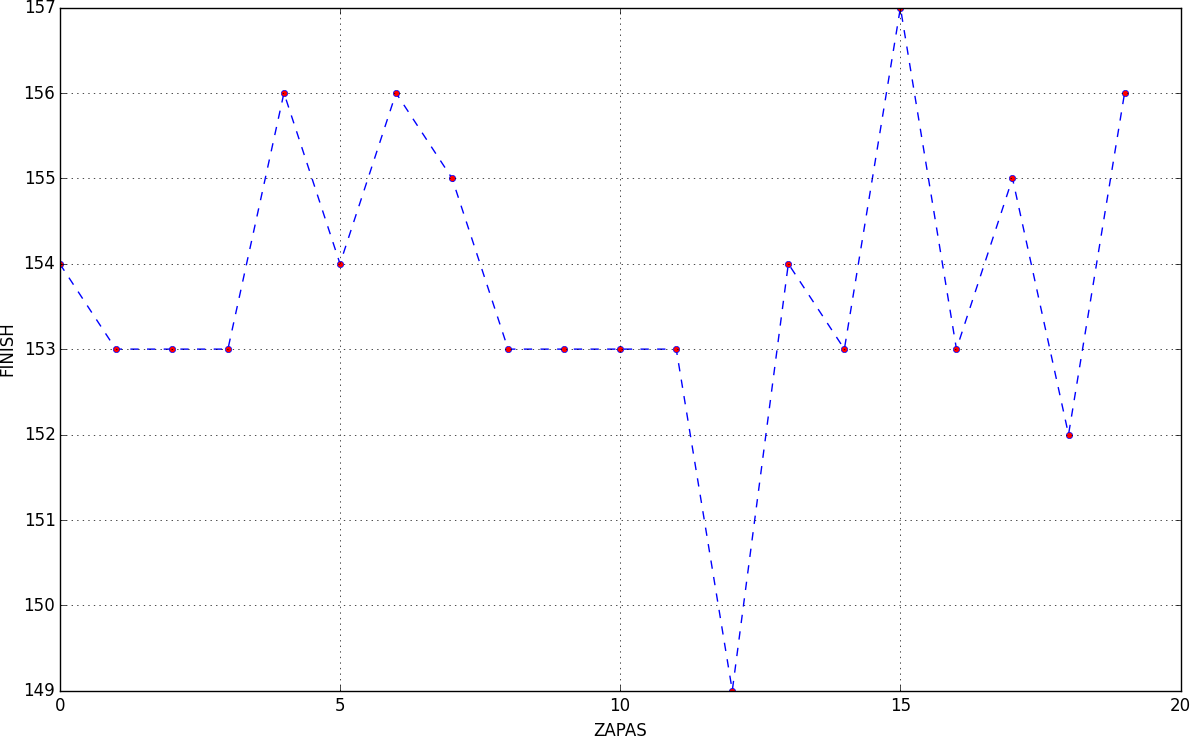
\includegraphics[width=150mm]{pic/modification_chart}
  \caption{Зависимость числа выпущенных изделий от \\
    значения порога заполнения бункера}
  \label{pic:modification_chart}
\end{figure}

Исходя из рисунка видно, что максимальное число выпущенных изделий 
приходится на тот случай, когда очередное заполнение бункера
производится при наличии в нем 15 килограммов сырья. 

Результаты модифицированной модели при оптимальном значении точки заказа
приведены в таблице~\ref{tbl:modified_result}.

\begin{table}[h!]
  \caption{Результаты модифицированной имитационной модели}
  \label{tbl:modified_result}
    \centering
    \begin{tabular}{| p{0.82\textwidth} | c |}
      \hline
      Величина & 
      Значение \\
      \hline

      Коэффициент загрузки первого нагревателя &
      0{,}262 \\
      \hline

      Коэффициент загрузки второго нагревателя &
      0{,}265 \\
      \hline

      Коэффициент загрузки третьего нагревателя &
      0{,}256 \\
      \hline

      Коэффициент загрузки формы &
      0{,}194 \\
      \hline

      Общее число выпущенных изделий &
      157 \\
      \hline

    \end{tabular}
\end{table}

Из неё видно, что эффективность модифицированной модели выше, чем базовой
(общее число выпущенных изделий --- 157 против 153).

Статистика модифицированной имитационной модели находится в приложении Б.